本节描述了常规GPU的工作原理,以及GPU与其他类型加速器的区别。\par

\hspace*{\fill} \par %插入空行
\textbf{GPU构建块}

图15-1展示了一个非常简化的GPU,由三个构建块组成:\par

\begin{itemize}
	\item 执行资源:GPU是执行计算工作的处理器。不同的GPU供应商对其执行资源使用不同的名称,所有现代GPU都由多个可编程处理器组成。处理器可以是异构和专门的,也可以是同构的。大多数现代GPU的处理器都是同构的。
	\item 固定功能:GPU是硬件单元,其可编程性低于执行资源,专门用于单个任务。当GPU用于图形时,图形管道的许多部分(如栅格化或光线追踪)都使用GPU来执行,以提高能效和性能。当GPU用于数据并行计算时,可能用于工作负载调度、纹理采样和依赖跟踪等任务。
	\item 缓存和内存:像其他处理器类型一样,GPU有缓存来存储执行资源访问的数据。GPU缓存可能是隐式的,不需要开发者做什么,或者显式的暂存存储器,开发者只要在使用数据之前,有目的地将数据移动到缓存中即可。许多GPU也有很大的内存池,来提供对执行资源使用数据的快速访问。
\end{itemize}

\hspace*{\fill} \par %插入空行
图15-1 常规GPU的构建块
\begin{center}
	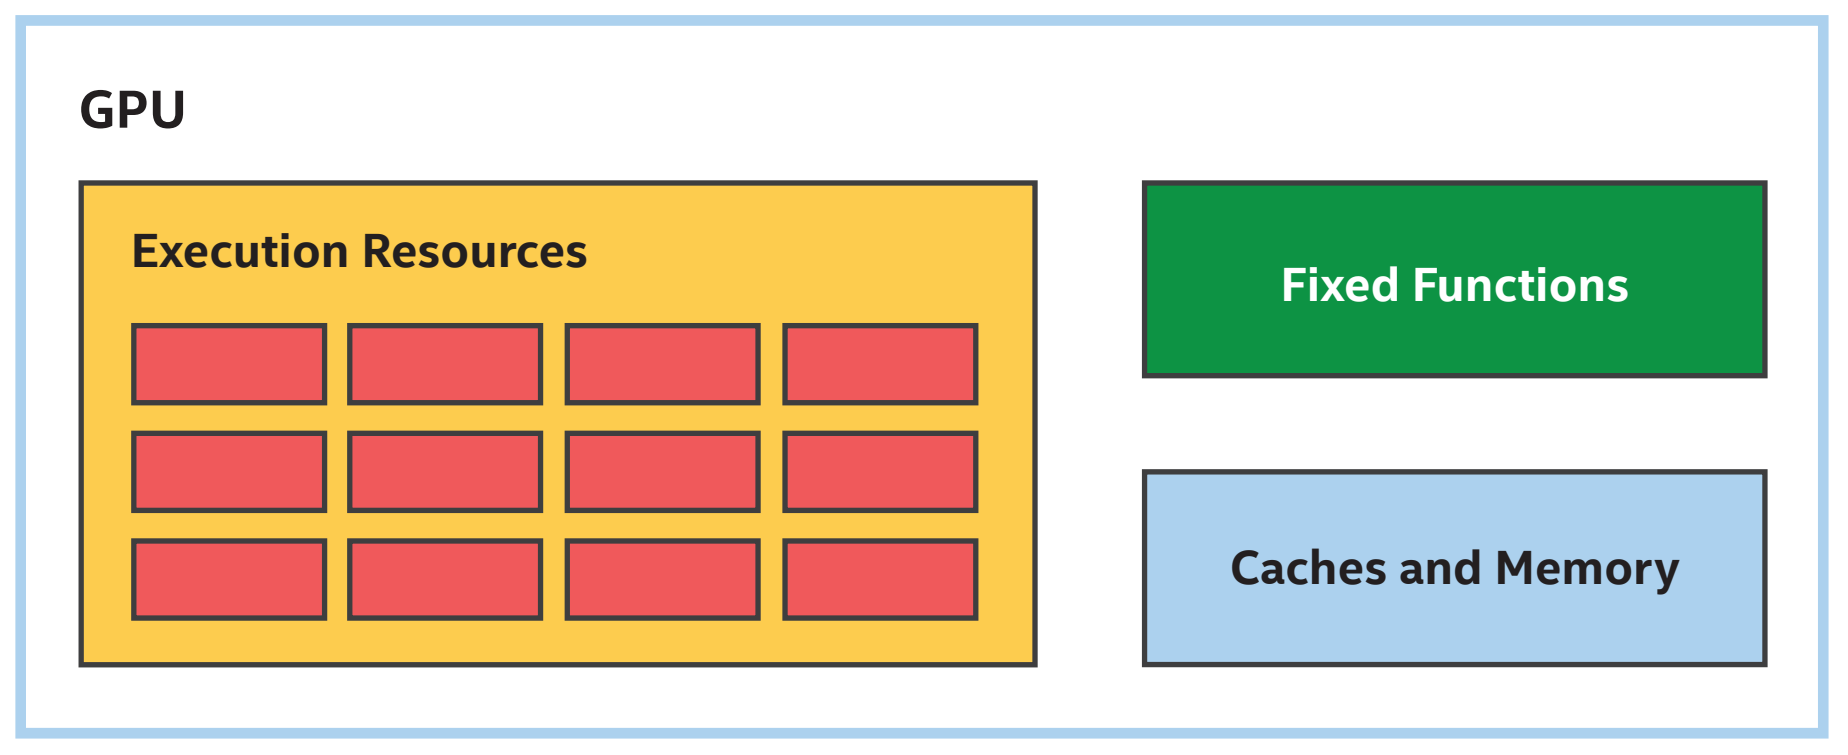
\includegraphics[width=1.0\textwidth]{content/chapter-15/images/2}
\end{center}

\hspace*{\fill} \par %插入空行
\textbf{更简单的处理器}

以前执行图形操作时,GPU处理大量数据。例如,游戏帧或渲染工作量涉及数千个顶点,这些顶点每帧产生数百万个像素。为了保持帧率,必须尽快处理这些大量数据。\par

常规GPU设计权衡是消除形成执行资源的处理器特性,从而加速单线程性能,并使用节省来资源进行额外的构建,如图15-2所示。例如,GPU处理器可能不包括复杂的乱序执行能力或其他类型处理器使用的分支预测逻辑。由于这些权衡,单个数据元素在GPU上的处理速度可能会比在其他处理器上慢,但更多的处理器数量使GPU能够快速有效地处理许多数据元素。\par

\hspace*{\fill} \par %插入空行
图15-2 GPU处理器更简单,但数量多
\begin{center}
	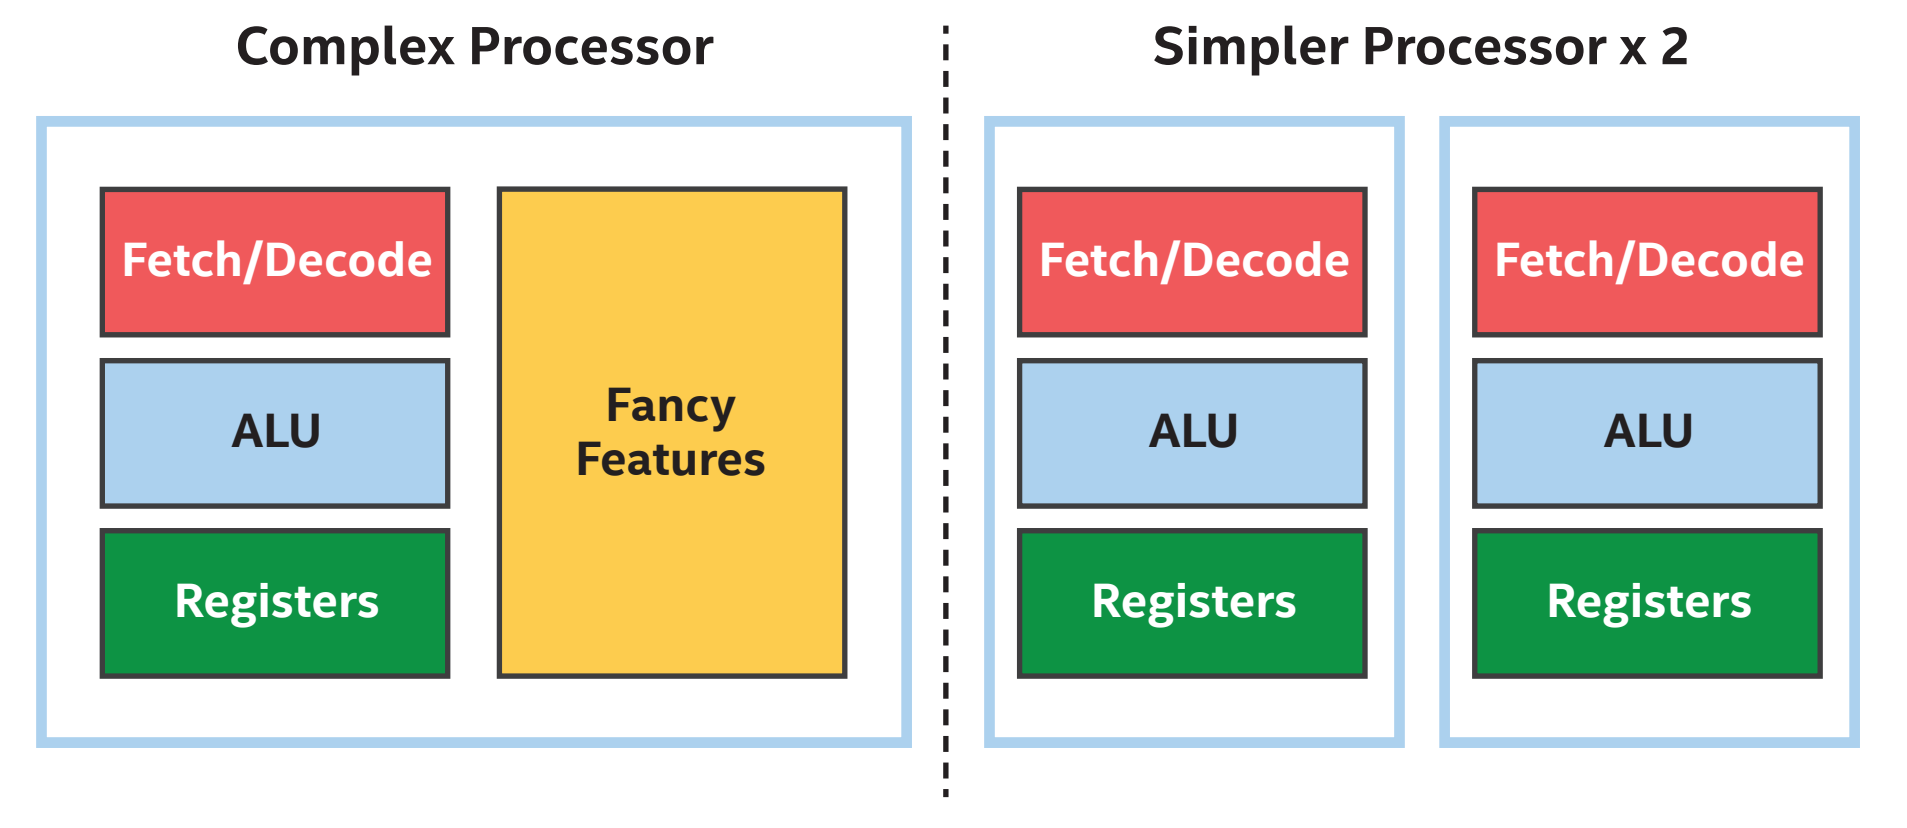
\includegraphics[width=1.0\textwidth]{content/chapter-15/images/3}
\end{center}

为了利用这种权衡,给GPU足够大的数据范围就很重要。为了说明加载大量数据的重要性,请参考本书中的矩阵乘法内核。\par

\begin{tcolorbox}[colback=blue!5!white,colframe=blue!75!black, title=关于矩阵乘法]
本书中,矩阵乘法内核用于演示内核中的更改或它的分配方式是如何影响性能的。虽然使用本章描述的技术可以显著提高矩阵乘法的性能,但矩阵乘法是如此重要和常见的操作,许多硬件(GPU、CPU、FPGA、DSP等)供应商已经实现了许多例程的高度调优版本,包括矩阵乘法。供应商投入大量的时间和精力来实现和验证特定设备的功能,在某些情况下可能会使用在标准内核中难以或不可能使用的功能或技术。
\end{tcolorbox}

\begin{tcolorbox}[colback=blue!5!white,colframe=blue!75!black, title=使用供应商提供的库!]
当供应商提供函数库实现时,使用它而不是重新实现内核!对于矩阵乘法,可以将oneMKL作为适合DPC++开发者的英特尔oneAPI解决方案工具包的一部分。
\end{tcolorbox}

矩阵乘法内核可以通过将其作为单个任务,提交到一个队列中,并在GPU上执行。这个矩阵乘法内核的主体,看起来就像在主机CPU上执行的函数,如图15-3所示。\par

\hspace*{\fill} \par %插入空行
图15-3 单个任务矩阵乘法看起来很像CPU主机代码
\begin{lstlisting}[caption={}]
h.single_task([=]() {
	for (int m = 0; m < M; m++) {
		for (int n = 0; n < N; n++) {
			T sum = 0;
			for (int k = 0; k < K; k++)
			sum += matrixA[m * K + k] * matrixB[k * N + n];
			matrixC[m * N + n] = sum;
		}
	}
});
\end{lstlisting}

如果尝试在CPU上执行这个内核,可能会执行得很好——如果不是很好,因为没利用CPU的并行能力,但对于较小的矩阵大小来说可能就足够了。如图15-4所示,如果试图在GPU上执行这个内核,可能会执行得非常糟糕,因为单个任务将只使用单个GPU处理器。\par

\hspace*{\fill} \par %插入空行
图15-4 GPU上的单个任务内核会使许多执行资源闲置
\begin{center}
	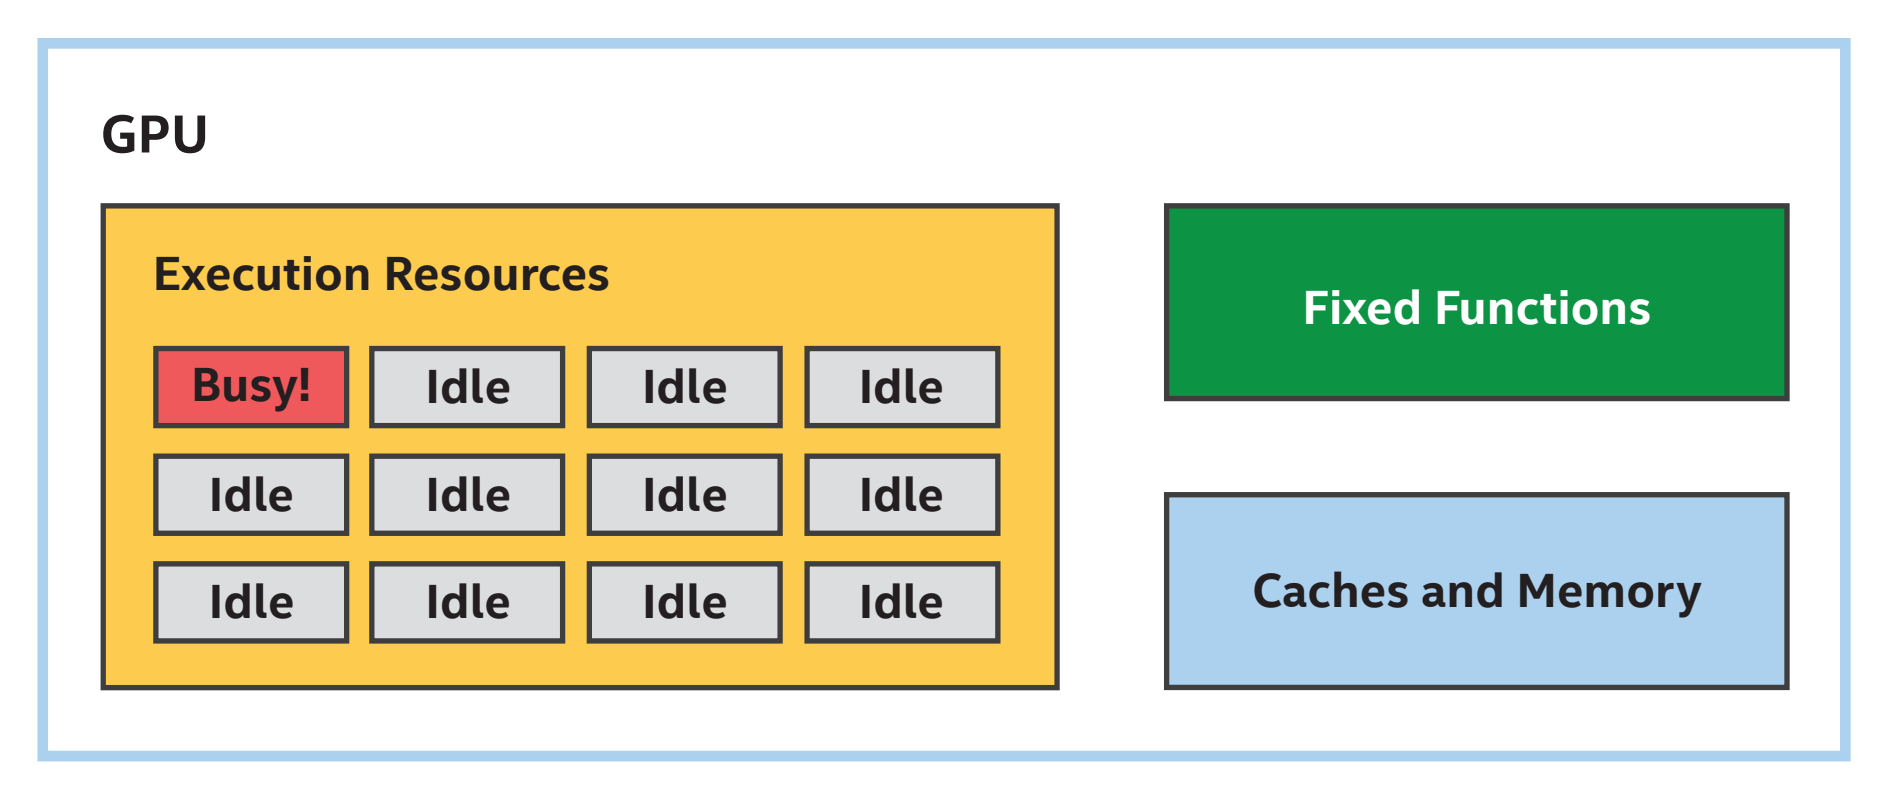
\includegraphics[width=1.0\textwidth]{content/chapter-15/images/4}
\end{center}

\hspace*{\fill} \par %插入空行
\textbf{表达并行性}

提高这个内核在CPU和GPU上的性能,可以通过将一个循环转换为parallel\_for来代替提交要并行处理的数据元素。对于矩阵乘法内核,可以选择提交表示两个最外层循环的数据元素。图15-5中,选择并行处理结果矩阵的行。\par

\hspace*{\fill} \par %插入空行
图15-5 类似矩阵乘法
\begin{lstlisting}[caption={}]
h.parallel_for(range{M}, [=](id<1> idx) {
	int m = idx[0];
	for (int n = 0; n < N; n++) {
		T sum = 0;
		for (int k = 0; k < K; k++)
		sum += matrixA[m * K + k] * matrixB[k * N + n];
		matrixC[m * N + n] = sum;
	}
});
\end{lstlisting}

\begin{tcolorbox}[colback=blue!5!white,colframe=blue!75!black, title=选择如何并行化]
选择并行化哪个维度是对GPU和其他设备类型调优的重要方法。本章的后续部分将描述,为什么在一个维度上并行比在不同维度上并行执行得更好。
\end{tcolorbox}

尽管并行内核与单任务内核非常相似,但应该在CPU上运行得更好,在GPU上运行得更好。如图15-6所示,paralle\_for使表示结果矩阵行的工作项能够在多个处理器资源上并行处理,因此所有执行资源都保持忙碌。\par

\hspace*{\fill} \par %插入空行
图15-6 某种程度上的并行内核使更多的处理器资源处于繁忙状态
\begin{center}
	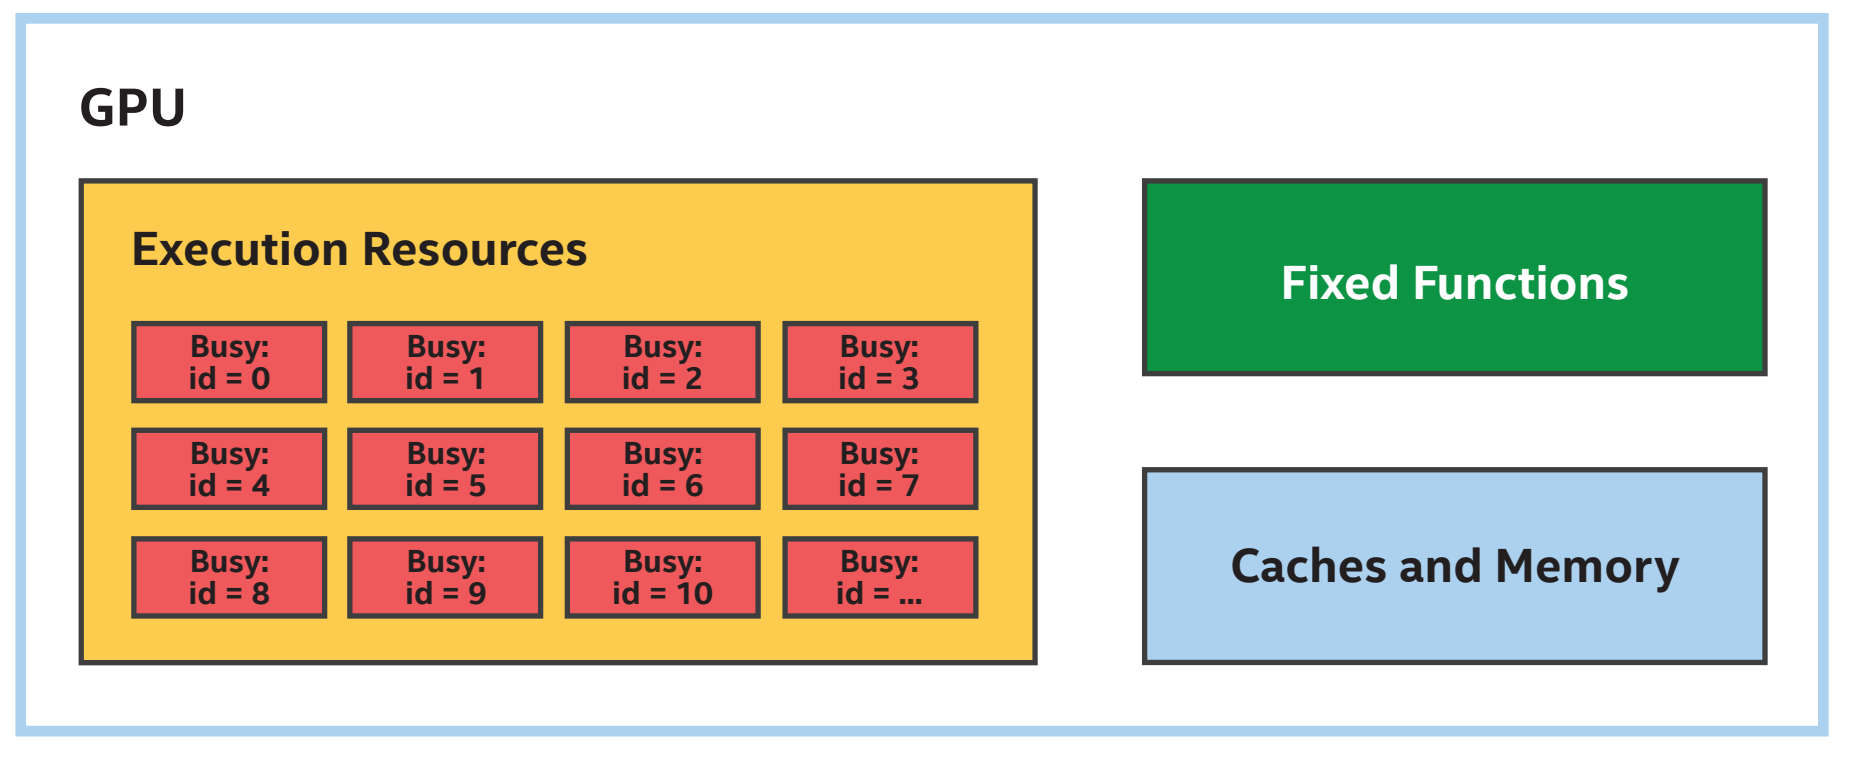
\includegraphics[width=1.0\textwidth]{content/chapter-15/images/5}
\end{center}

注意,没有指定将行分区并分配给不同处理器资源的确切方式,这为选择在设备上执行内核提供了灵活性。例如,可以选择在同一个处理器上执行连续的行,而不是在处理器上执行单个行,以利用局域性。\par

\hspace*{\fill} \par %插入空行
\textbf{表达更多的并行性}

通过选择并行处理两个外部循环,可以将矩阵乘法内核更加的并行化。因为paralle\_for可以表示最多三个维度上的并行循环,如图15-7所示。图中,传递给paralle\_for的范围和表示并行执行空间中索引的项都是二维的。\par

\hspace*{\fill} \par %插入空行
图15-7 更多的并行矩阵乘法
\begin{lstlisting}[caption={}]
h.parallel_for(range{M, N}, [=](id<2> idx) {
	int m = idx[0];
	int n = idx[1];
	T sum = 0;
	for (int k = 0; k < K; k++)
		sum += matrixA[m * K + k] * matrixB[k * N + n];
	matrixC[m * N + n] = sum;
});
\end{lstlisting}

在GPU上运行时,并行性可能会提高矩阵乘法内核的性能。即使当矩阵的行数超过GPU处理器的数量时,这也可能是正确的。接下来的几节将描述这种情况的原因。\par

\hspace*{\fill} \par %插入空行
\textbf{简化控制逻辑(SIMD指令)}

许多GPU处理器通过大多数数据元素在内核中采用相同的控制流路径来优化控制逻辑。例如,在矩阵乘法内核中,每个数据元素执行最内层循环的次数相同,因为循环边界不变。\par

当数据元素以相同的控制流通过内核时,处理器可以通过在多个数据元素之间共享控制逻辑,并将它们作为一个组来执行来降低管理指令流的成本。一种方法是实现单指令、多数据或SIMD指令集,其中多条数据元素由一条指令同时处理。\par

\begin{tcolorbox}[colback=blue!5!white,colframe=blue!75!black, title=线程与指令流]
在许多并行编程上下文中和GPU文献中,术语“线程”用来表示“指令流”。上下文中,“线程”与传统的操作系统线程不同,通常更轻量级。但情况并非总是如此,在某些情况下,“线程”用来描述完全不同的东西。\\

由于术语“线程”是重载的,很容易误解,本章使用术语“指令流”代替。
\end{tcolorbox}

\hspace*{\fill} \par %插入空行
图15-8 4个宽SIMD处理器:4个ALU共享取/解码逻辑
\begin{center}
	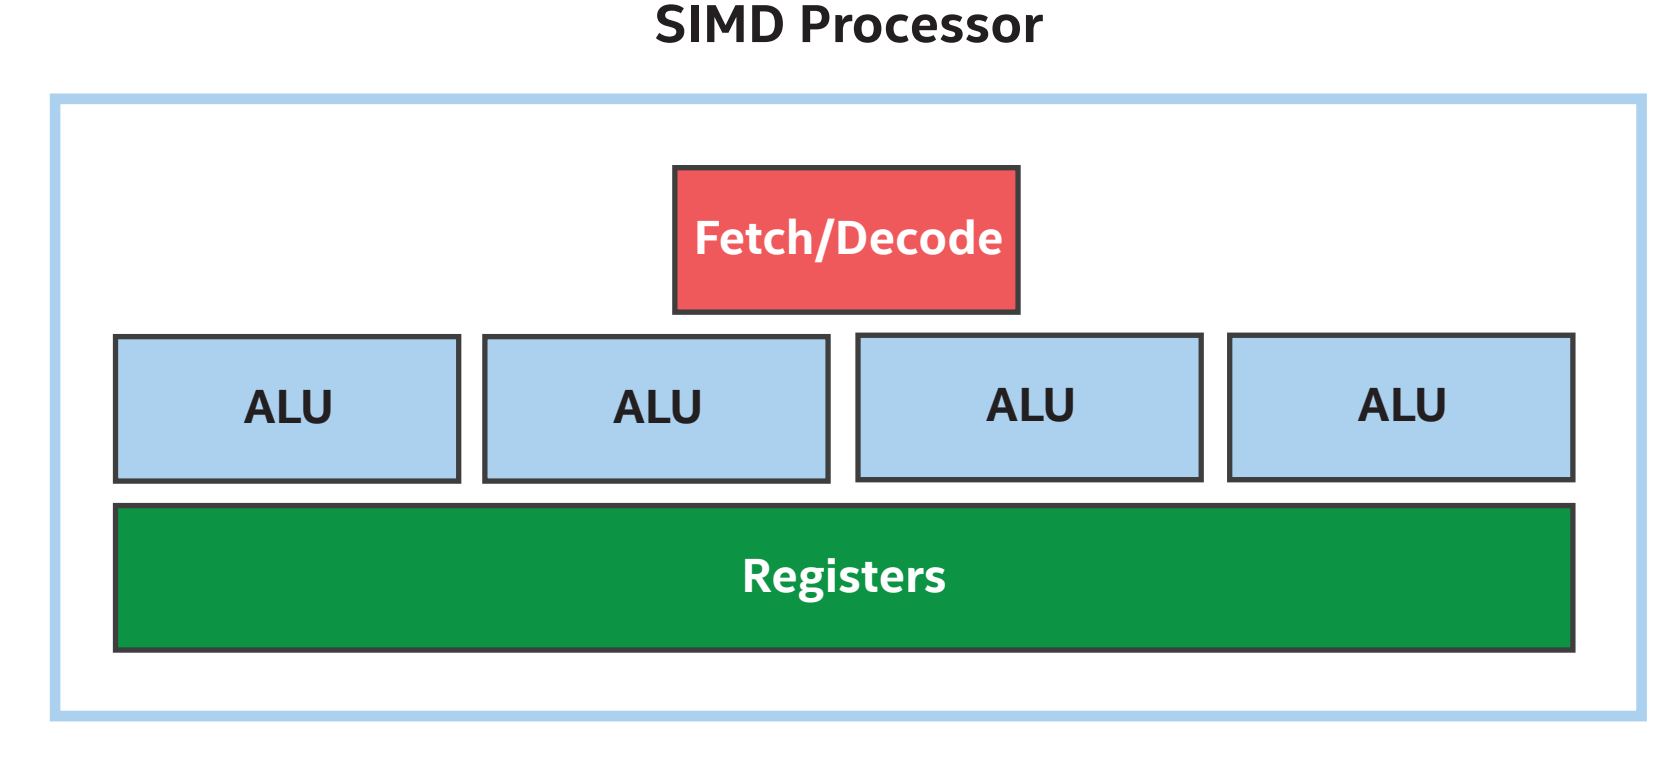
\includegraphics[width=1.0\textwidth]{content/chapter-15/images/6}
\end{center}

单个指令同时处理的数据元素的数量,有时称为指令的SIMD宽度或执行指令的处理器。图15-8中,4个ALU共享相同的控制逻辑,因此可以将其描述为一个宽度为4的SIMD处理器。\par

GPU并不是唯一实现SIMD指令集的处理器。其他处理器类型也实现了SIMD指令集,以提高处理大型数据集时的效率。GPU和其他处理器类型之间的主要区别是,GPU依赖于并行执行多个数据元素来获得良好的性能,而且GPU可能比其他处理器类型支持更宽的SIMD宽度。例如,GPU支持16、32或更多数据元素的SIMD宽度并不少见。\par

\begin{tcolorbox}[colback=blue!5!white,colframe=blue!75!black, title=编程模型:SPMD和SIMD]
虽然GPU实现不同宽度的SIMD指令集,但这通常是实现细节,并且对在GPU上执行数据并行内核的应用程序是透明的。这是因为许多GPU编译器和运行时API实现了单程序、多数据或SPMD编程模型,其中GPU编译器和运行时API决定用SIMD指令流处理最有效的一组数据元素,而不是显式地表达为SIMD指令。第9章的“子工作组”一节探讨了数据元素分组对应用程序可见的情况。
\end{tcolorbox}

图15-9扩展了执行资源,以支持宽度为4的SIMD,允许并行处理四倍的矩阵行。\par

\hspace*{\fill} \par %插入空行
图15-9 SIMD处理器上执行并行的内核
\begin{center}
	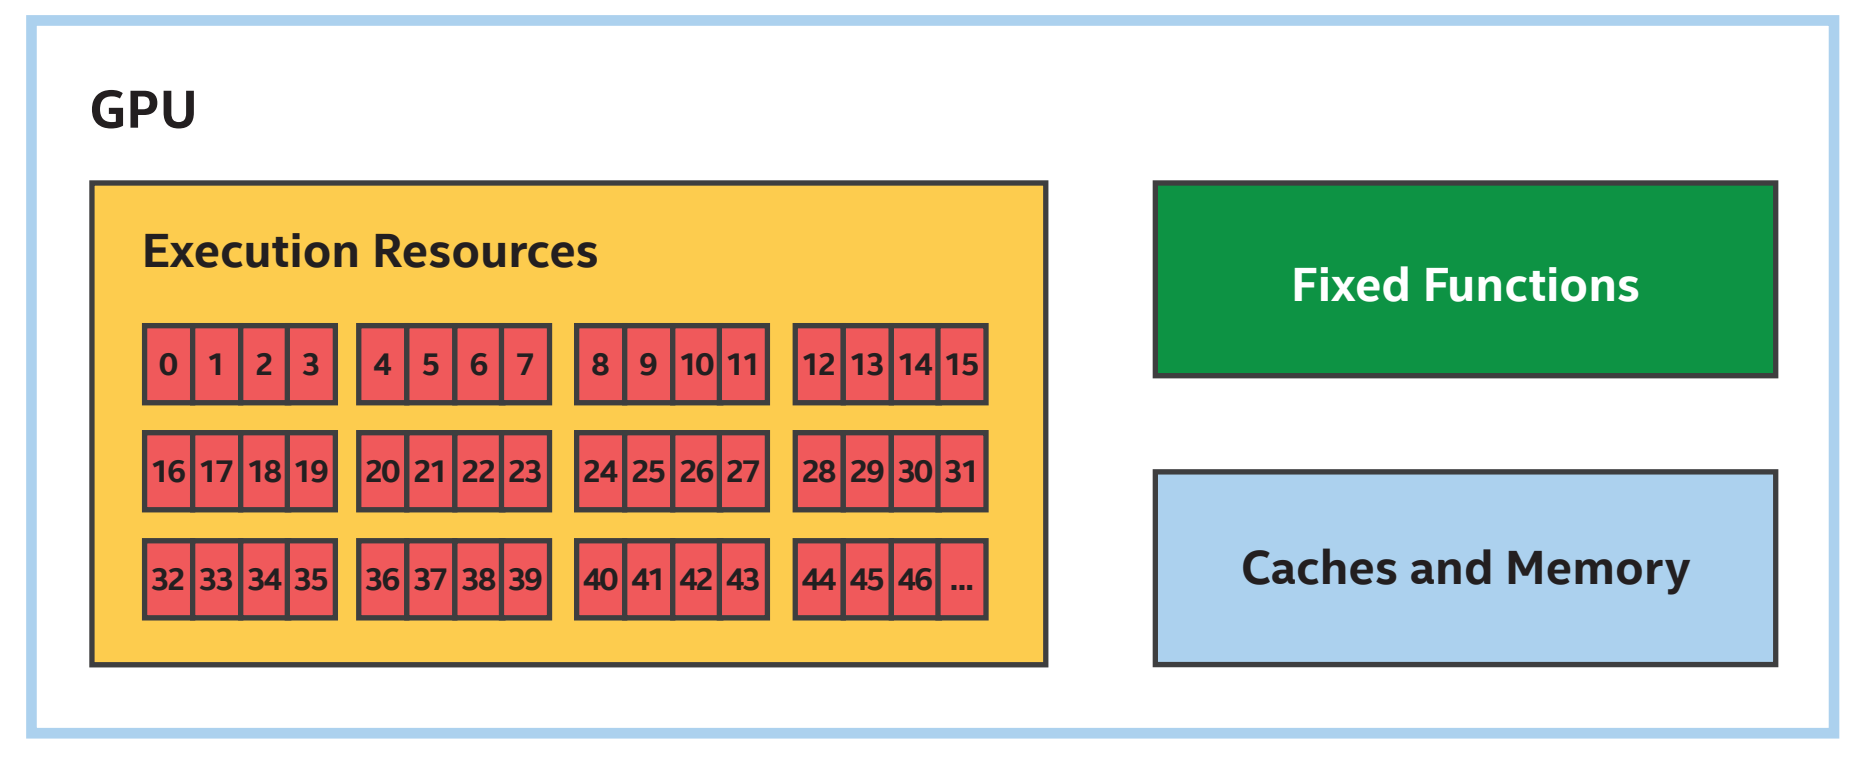
\includegraphics[width=1.0\textwidth]{content/chapter-15/images/7}
\end{center}

通过使用并行处理多个数据元素的SIMD指令,图15-5和15-7中的并行矩阵乘法内核的性能可以超越单个处理器的数量。通过在同一个处理器上执行连续的数据元素,SIMD指令的使用还在许多情况下提供了局域性优势,包括矩阵乘法。\par

\begin{tcolorbox}[colback=red!5!white,colframe=red!75!black]
内核受益于处理器之间的并行性和处理器内部的并行性!
\end{tcolorbox}

\hspace*{\fill} \par %插入空行
\textbf{预测和屏蔽}

只要在内核中所有数据元素通过相同的路径通过条件代码,那么在多个数据元素之间共享指令流就可以很好地工作。当数据元素在条件代码中采取不同的路径时,控制流称为分叉。当控制流在SIMD指令流中分叉时,通常执行两个控制流路径,并屏蔽或预测一些通道。这确保了正确的行为,但是这种正确性以性能为代价,因为屏蔽的通道不会执行有用的操作。\par

为了展示预测和屏蔽是如何工作的,请考虑图15-10中的内核,将具有“奇数”索引的每个数据元素乘以2,并将具有“偶数”索引的每个数据元素加1。\par

\hspace*{\fill} \par %插入空行
图15-10 具有发散控制流的内核
\begin{lstlisting}[caption={}]
h.parallel_for(array_size, [=](id<1> i) {
	auto condition = i[0] & 1;
	if (condition)
		dataAcc[i] = dataAcc[i] * 2; // odd
	else
		dataAcc[i] = dataAcc[i] + 1; // even
});
\end{lstlisting}

假设在图15-8所示的宽度为4的SIMD处理器上执行这个内核,并且在一个SIMD指令流中执行前4个数据元素,在不同的SIMD指令流中执行接下来的4个数据元素,以此类推。图15-11显示了屏蔽通道和预测执行的一种方式,正确地使用不同的控制流执行了这个内核。\par

\hspace*{\fill} \par %插入空行
图15-11 发散型内核可能的通道掩码
\begin{center}
	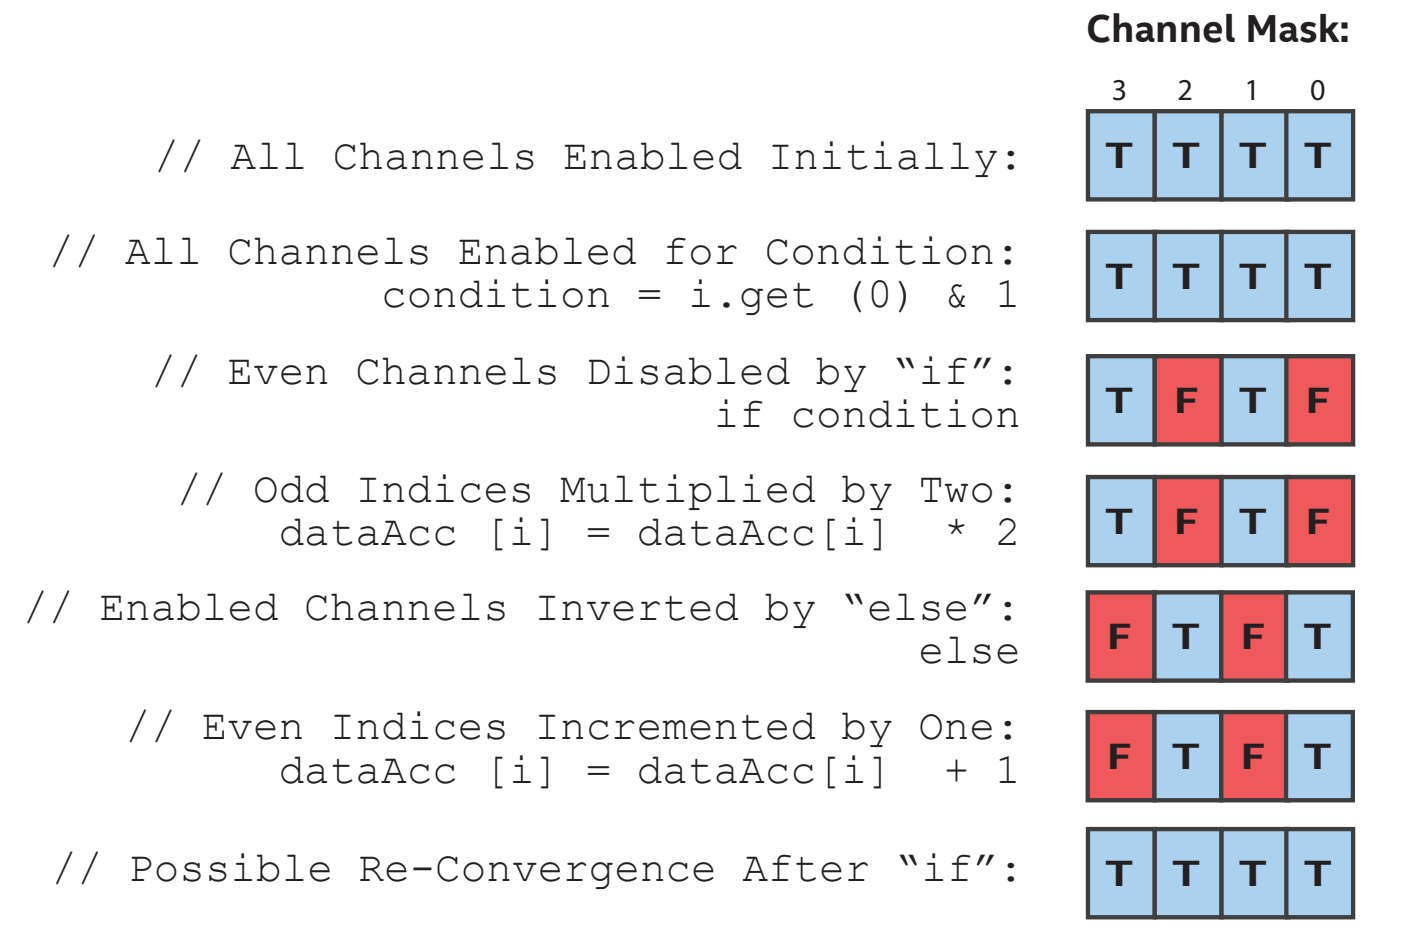
\includegraphics[width=1.0\textwidth]{content/chapter-15/images/8}
\end{center}

\hspace*{\fill} \par %插入空行
\textbf{SIMD效率}

SIMD效率度量的是与等效标量指令流相比SIMD指令流执行得有多好。图15-11中,由于控制流将通道划分为两个相等的组,所以发散控制流中的每条指令执行效率只有一半。最坏的情况下,对于高度分散的内核,效率可能会降低。\par

所有实现SIMD指令集的处理器都会受到影响SIMD效率的差异惩罚,但因为GPU通常比其他处理器类型支持更宽的SIMD,当优化GPU的内核时,重新构造算法来最小化不同的控制流和最大化融合执行可能特别有用。但也并不总是可以这样做,选择以更收敛的执行并行化维度,可能比以高度发散的执行并行化另一个维度执行要好。\par

\hspace*{\fill} \par %插入空行
\textbf{SIMD效率和组中工作项}

目前为止,本章中的所有内核都是基本的数据并行内核,没有在执行范围内指定任何项目分组,这给了实现为设备选择最佳分组的机会。例如,具有较宽SIMD的设备可能更喜欢较大的分组,具有较窄SIMD的设备可能适合较小的分组。\par

当内核具有明确工作项分组的ND-Range内核时,应该注意选择能够最大化SIMD效率的ND-Range工作组大小。当工作组的大小不能被处理器的SIMD宽度整除时,部分工作组可能会在内核的整个过程中禁用通道。可以使用preferred\_work\_group\_size\_multiple查询来选择有效的工作组大小。关于如何查询设备属性的更多信息,请参阅第12章。\par

选择包含单个工作项的工作组大小可能会表现得非常糟糕,因为许多GPU将通过屏蔽除其他所有SIMD通道来实现单个工作项工作组。例如,图15-12中的内核可能比图15-5中非常相似的内核性能要差得多,两者之间唯一显著的区别是从一个基本的数据并行内核,改为一个低效的单工作项ND-Range内核(nd\_range<1>\{M, 1\})。\par

\hspace*{\fill} \par %插入空行
图15-12 低效的单项矩阵乘法
\begin{lstlisting}[caption={}]
// A work-group consisting of a single work-item is inefficient!
h.parallel_for(nd_range<1>{M, 1}, [=](nd_item<1> idx) {
	int m = idx.get_global_id(0);
	
	for (int n = 0; n < N; n++) {
		T sum = 0;
		for (int k = 0; k < K; k++)
			sum += matrixA[m * K + k] * matrixB[k * N + n];
		matrixC[m * N + n] = sum;
	}
});
\end{lstlisting}

\hspace*{\fill} \par %插入空行
\textbf{切换工作以隐藏延迟}

许多GPU实现了另一种技术来简化控制逻辑,最大化执行资源,并提高性能:许多GPU允许多个指令流同时驻留在一个处理器上,而不是在处理器上执行单个指令流。\par

处理器上驻留多个指令流利于性能,可以让处理器选择要执行的工作。如果指令流执行了长延迟的操作,比如:从内存读取,处理器可以切换并运行的不同指令流,而不是阻塞等待操作完成。有了足够的指令流,当处理器切换回原始指令流时,长延迟的操作可能已经完成,而不需要处理器阻塞等待。\par

图15-13展示了处理器如何使用多个并发指令流,来隐藏延迟并提高性能。尽管第一个指令流在多个指令流中执行的时间要长一些,但通过切换到其他指令流,处理器能够找到准备执行的工作,而不需要等待长操作完成。\par

\hspace*{\fill} \par %插入空行
图15-13 切换指令流以隐藏延迟
\begin{center}
	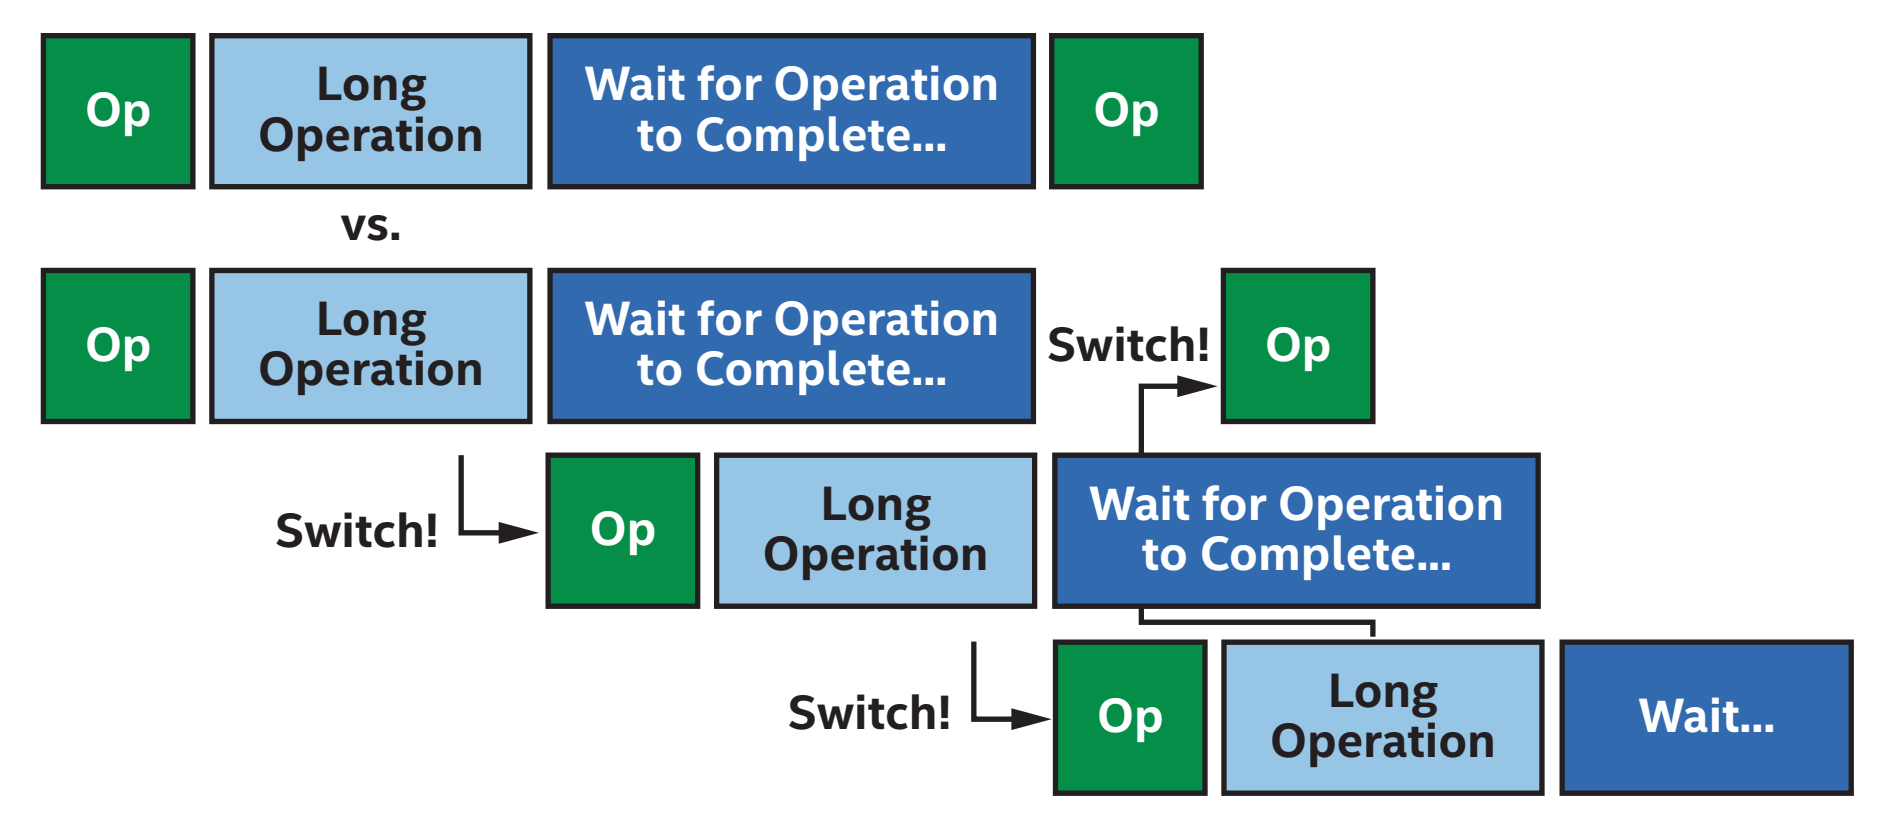
\includegraphics[width=1.0\textwidth]{content/chapter-15/images/9}
\end{center}

GPU分析工具可以使用占用率等术语,来描述GPU处理器当前执行的指令流数量与理论指令流总数的对比。\par

低占用率并不一定意味着低性能,因为少量指令流可能会使处理器繁忙。同样,高占用率并不一定意味着高性能,因为如果所有指令流执行低效的、长延迟的操作,GPU仍然需要等待。其他条件相同的情况下,增加占用率可以最大化GPU隐藏延迟的能力,通常也会提高性能。增加占用率是图15-7中并行的内核提高性能的另一个原因。\par

这种在多个指令流之间切换,以隐藏延迟的技术特别适合于GPU和数据并行处理。从图15-2中可以看出,GPU通常比其他处理器更简单,因此缺乏复杂的延迟隐藏特性。这使得GPU更容易受到延迟问题的影响,但是由于数据并行编程涉及到处理大量的数据,GPU通常有大量指令流要执行!\par














